\chapter{EXPLOITING GPU}\label{exploitinggpu}
\section{Background}
\subsection{Prior Work}
ACESIII supported exploitation of GPUs. However, the SIAL programmer has to deal
with a lot of low-level GPU memory operations such as allocating memory on GPU,
copying blocks to and from GPU and deallocating memory on GPU. Since not all
calculations are suitable to be executed on GPU, the SIAL programmer has to explicitly mark
regions of SIAL code suitable for execution on GPU.

\begin{lstlisting}[caption={Code fragment from ACESIII for CCSD calculation},
  label={lst:ACESIII_gpucode}]
#start of GPU region
gpu_begin
#allocate and initialize blocks on GPU
gpu_put aoint(lambda,mu,sigma,nu) #allocate and copy data from CPU
DO i1
DO j1
    gpu_put LT2AOab1(mu,i1,nu,j1)
    gpu_put LT2AOab2(nu,j1,mu,i1)
    gpu_put LTAOab(lambda,i1,sigma,j1)
ENDDO j1
ENDDO i1
gpu begin
DO i
DO j
    #perform computations on GPU
    Yab(mu,i,nu,j) = 0.0
    Y1ab(nu,j,mu,i) = 0.0
    gpu_allocate Yab(mu,i,nu,j) # allocate temp blocks on GPU
    gpu_allocate Y1ab(nu , j ,mu, i )
    #contraction Y1ab(nu,j,mu,i) = Yab(mu,i,nu,j) #permutation
    Yab(mu,i,nu,j) = aoint(lambda,mu,sigma,nu)*LTAOab(lambda,i,sigma,j)
    LT2AOab1(mu,i,nu,j) += Yab(mu,i,nu,j) #element−wise sums
    LT2AOab2(nu,j,mu,i) += Y1ab(nu,j,mu,i) #element−wise sums
    gpu_free Yab(mu,i,nu,j) #free temp blocks on GPU
    gpu_free Y1ab(nu,j,mu,i)
ENDDO j
ENDDO i
#copy results to CPU , free blocks on GPU
DO i1
DO j1
    gpu_get LT2AOab1(mu,i1,nu,j1)
    gpu_get LT2AOab2(nu,j1,mu,i1)
    gpu_free LT2AOab1(mu,i1,nu,j1)
    gpu_free LT2AOab2(nu,j1,mu,i1)
    gpu_free LTAOab(lambda,i1,sigma,j1)
ENDDO j1
ENDDO i1
gpu_free aoint(lambda,mu,sigma,nu)
gpu_end
#end of GPU region
\end{lstlisting}

A code fragment from ACESIII for CCSD calculation is presented
in~\ref{lst:ACESIII_gpucode}. In line 2 and 39, the region is marked to be executed
on GPU and blocks of lines 5-11 and 29-37 deal with managing memory to and from
GPU and host memory. The actual calculations are done by lines 13-27.

\section{GPU Support in ACES4}
The rest of this chapter describes how the support for GPUs in ACES4 was improved
by providing automatic memory management and techniques devised to optimally transfer
the data between the GPU memory and the host memory.

\section{Unoptimized Runtime Memory Management}
To manage the block memory and to automate the memory transfer between GPU and CPU,
metadata about the state of memory is stored in the interpreter. The \texttt{Block} class
which represents the SIA \textit{block} in the interpreter was modified to now store
this metadata and pointer to the memory location in GPU and host memory in form of
an object of another class \texttt{Device\_Info}.

Due to this additional layer, supporting multiple compute devices is now possible.
The metadata includes flags for block data being \textit{valid}.
It also includes a field, \textbf{version number}, which is incremented each time the block is changed
by the compute device. This helps in keeping memory of different compute devices
synchronized.

\begin{lstlisting}[caption={\texttt{Device\_Info} class structure},
  language=C++,
  label={lst:deviceinfostructure}]
class DeviceInfo {
  double* data_ptr_;
  unsigned int data_version_;
  bool isAsync;  // are there any pending operations on device
}
\end{lstlisting}

The code shown in~\ref{lst:deviceinfostructure} is one of the ways of expressing
the class \texttt{Device\_Info} in C++ language.

\begin{figure}[h] %place figure "here"
  \centering

  \tikzstyle{table}=[
  matrix of nodes,
  row sep=-\pgflinewidth,
  column sep=-\pgflinewidth,
  nodes={typetag}]
  \begin{tikzpicture}[list/.style={rectangle split, rectangle split parts=3,
      draw, rectangle split horizontal,align=center}, >=stealth, start chain,
    container/.style={draw=gray, inner sep=1ex},
    typetag/.style={draw=none, anchor=west},
    title/.style={draw=none, color=gray, inner sep=0pt}]

    \matrix[table] (block)
    {
      |[title]|Block  &            \\
      {BlockId}       & {$\dotsb$} \\
      {BlockShape}    & {$\dotsb$} \\
      {BlockSelector} & {$\dotsb$} \\
      {Devices:}      & |[list]|   \\
    };

    \matrix[table, below=of block] (CPU_device)
    {
      |[title]|Device\_Info    &            \\
      {\texttt{data\_version}} & {$\dotsb$} \\
      {\texttt{isAsync}}       & {$\dotsb$} \\
      {\texttt{data}}          & {}         \\
    };

    \matrix[table, right=of CPU_device] (GPU_device)
    {
      |[title]|Device\_Info    &            \\
      {\texttt{data\_version}} & {$\dotsb$} \\
      {\texttt{isAsync}}       & {$\dotsb$} \\
      {\texttt{data}}          & {}         \\
    };

    \node[container, fit=(block)] {};
    \node[container, fit=(CPU_device)] {};
    \node[container, fit=(GPU_device)] {};

    \node[inner sep=0pt, below=of CPU_device] (cpu-mem)
    {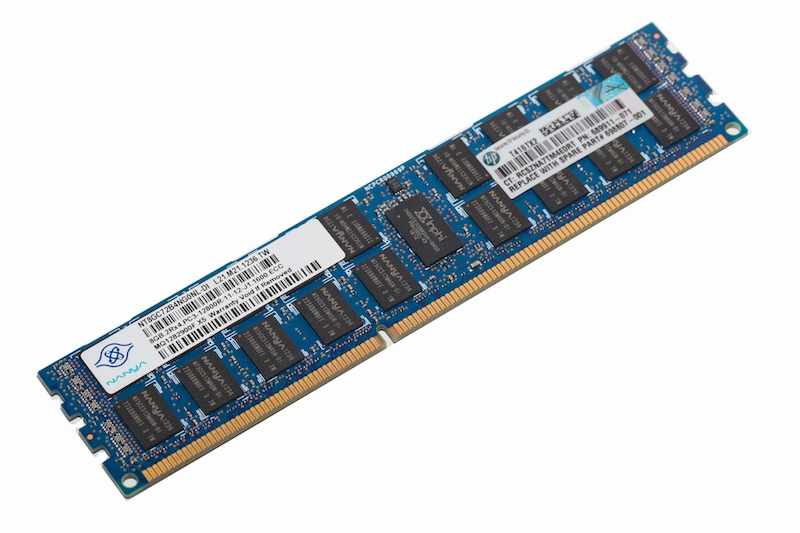
\includegraphics[width=.25\textwidth]{images/cpu-mem.jpg}};

    \node[inner sep=0pt, right=of cpu-mem] (gpu-mem)
    {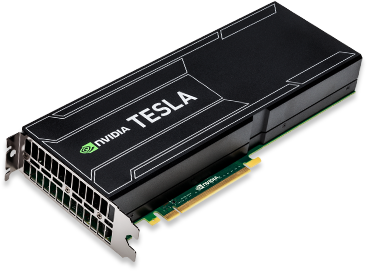
\includegraphics[width=.25\textwidth]{images/gpu-card.png}};

    \draw[*->] let \p1 = (block-5-2.one), \p2 = (block-5-2.center) in (\x1,\y2)    -- (CPU_device);
    \draw[*->] let \p1 = (block-5-2.second), \p2 = (block-5-2.center) in (\x1,\y2) -- (GPU_device);

    \draw[*->] (CPU_device-4-2.center) -- (cpu-mem);
    \draw[*->] (GPU_device-4-2.center) -- (gpu-mem);
  \end{tikzpicture}
  \caption{\texttt{Block} and \texttt{Device\_Info} structure}\label{fig:Device_Info_Structure}
\end{figure}

Using this metadata, specifically \texttt{data\_version\_}, the runtime can keep
track of changes to data by different devices and find the device with the latest
data by comparing version numbers:

\begin{algorithm} {Block::get\_latest\_device() $\rightarrow$ Device\_Info}
  \singlespacing

  \begin{algorithmic}[1]
    \Function{Block::get\_latest\_device}{}
    \State $highest\_version\_found \gets 0$
    \State $highest\_version\_device \gets null$
    \ForAll{$device\_info\ in\ this.devices$}
    \If{$device\_info.data\_version > highest\_version\_found$}
    \State {$highest\_version\_found \gets info.data\_version$}
    \State {$highest\_version\_device \gets device\_info$}
    \EndIf
    \EndFor
    \State \Return $highest\_version\_device$
    \EndFunction
    % \hline
  \end{algorithmic}
\end{algorithm}

After determining the device with latest version of data, the runtime can update
other devices, if needed. The only interfacing function exposed outside of
\texttt{Block} class is \texttt{get\_data(deviceid)} which returns a pointer to the memory
location on the device identified by \texttt{deviceid}. The logic to always return
the latest version of data can be embedded into \texttt{get\_data(device)}:

\begin{algorithm}  {Block::get\_data(deviceid) $\rightarrow$ double*}
  \singlespacing

  \begin{algorithmic}[1]
    \Function{Block::get\_data}{deviceid}
    \State $latest\_device \gets this.get\_latest\_device()$
    \If{$latest\_device.data\_version > this.devices[deviceid].data\_version$}
    \State {$memcpy(latest\_device.data,\ this.devices[deviceid].data)$}
    \State {$this.devices[deviceid].data\_version \gets latest\_device.data\_version$}
    \EndIf
    \State \Return $this.devices[deviceid].data$
    \EndFunction
    % \hline
  \end{algorithmic}
  \label{alg:get_data}
\end{algorithm}

\section{Optimizing Block Copying}
An enormous cost has to be paid~\cite{Bakkum2010, memorytransferoverhead}
for transferring memory to GPU as compared to the time taken for actual computation
on GPU. Hence, to have significant speed gains by executing on GPU over CPU,
it is necessary to minimize the time spent on block transfers. This has been
achieved by deploying multiple optimizations that are explained in this section.

\subsection{Reducing Block Transfers}
The first optimization includes saving unnecessary block synchronizations by
exploiting the semantics of SIAL. The runtime has information about whether each of
the parameter passed to builtin super instructions is going to be read, written or updated.
When each element of a block is modified, it is defined as block writing. Whereas,
if only some of the elements of a block are modified, then it is defined as block updating.
The runtime also has this information for the user defined super instructions, through
the user provided attributes, describing the intent for each parameter.
In listing~\ref{lst:userdefinedsuperinstructionattr}, we can see for the user
defined super instruction \texttt{fill\_block\_sequential} and the attributes \texttt{wr}.
This denotes that the first parameter passed to \texttt{fill\_block\_sequential}
is going to be written and the second is going to be read.

\begin{lstlisting}[caption={SIAL fragment showing user defined super instruction attributes},
  language=Fortran,
  label={lst:userdefinedsuperinstructionattr}]
sial contract_to_scalar
  predefined int norb
  special fill_block_sequential wr
  special fill_block_cyclic wr
  special print_block r
  special print_static_array r
  aoindex i = 1:1
  aoindex j = 1:1
  temp  a[i,j]
  ...
\end{lstlisting}

Using this information about the intent of each block request, the
number of synchronizations between devices can be reduced. Blocks which are
going to be written need not be synchronized, however, blocks requested for
being read or updated need to be synchronized for the requested device.

The algorithm presented in~\ref{alg:get_data} can be split into
\texttt{get\_data} and an explicit \texttt{update\_data}:

\begin{algorithm}  {Block::get\_data(deviceid) $\rightarrow$ double*}
  \singlespacing

  \begin{algorithmic}[1]
    \Function{Block::get\_data}{deviceid}
    \State \Return $this.devices[deviceid].data$
    \EndFunction
    \\
    \Function{Block::update\_data}{deviceid}
    \State $latest\_device \gets this.get\_latest\_device()$
    \If{$latest\_device.data\_version > this.devices[deviceid].data\_version$}
    \State {$memcpy(latest\_device.data,\ this.devices[deviceid].data)$}
    \State {$this.devices[deviceid].data\_version \gets latest\_device.data\_version$}
    \EndIf
    \State \Return $this$
    \EndFunction
    % \hline
  \end{algorithmic}
\end{algorithm}

With this change, the runtime can decide whether synchronizing block contents
is necessary. If the synchronization is needed, it can call
\texttt{block\-->update\_data(device)\-->get\_data(device)}
which is the case with block read and update. If no synchronization is needed, as in case
of a block being written, the runtime can simply get the pointer on device memory by calling
\texttt{block->get\_data(device)}.
This change in the way of accessing and updating block data along with the information
about the intent of the request can reduce several unnecessary synchronizations.

\subsection{Memory Pinning}\label{memory_pinning}
The memory allocated on CPU or host memory is pageable by default. GPUs cannot
access data on such pageable host memory~\cite{datatransferoptimization, programmingguidecuda}
directly. For this reason, when a memory copy operation is requested
from a host to a GPU, the CUDA driver first allocates a temporary \textbf{page locked},
or \textit{pinned}, memory on the host (host memory), copies the host memory to the
temporary pinned memory and then finally transfers the data from pinned memory
to GPU device memory.
\begin{figure}[h] %place figure "here"
  \begin{tikzpicture}[
    container/.style={draw=gray, inner sep=5mm},
    typetag/.style={draw=black, anchor=west, inner sep=2mm, text width=3cm},
    title/.style={draw=none, color=gray, inner sep=0pt}]

    \node[title]   (gpu-title)     at (0, 5) {GPU};
    \node[typetag] (gpu-ram)       at (0, 4) {DRAM};
    \node[title]   (cpu-title)     at (0, 2) {CPU};
    \node[typetag] (pinned)        at (0, 1) {Temporary Pinned Memory};
    \node[typetag] (main-pageable) at (4, 1) {Pageable Memory};

    \node[container, fit=(gpu-title)(gpu-ram)]               {};
    \node[container, fit=(cpu-title)(main-pageable)(pinned)] {};

    \draw[draw=black, solid, line width=1mm, fill=black,
    preaction={-triangle 90, thin, draw, shorten >=-1mm}] (main-pageable) -- (pinned.east);
    \draw[draw=black, solid, line width=1mm, fill=black,
    preaction={-triangle 90, thin, draw, shorten >=-1mm}] (pinned)        -- (gpu-ram.south);
  \end{tikzpicture}
  \caption{\texttt{memcpy} w/o memory pinning}\label{fig:wo_mem_pin}
\end{figure}

Due to this copying of data to a temporary page-locked memory, extra time
is spent in the redundant copy operation. To overcome this, page locked memory
can directly be allocated on the host memory. For this CUDA gives API \texttt{cudaMallocHost()},
\texttt{cudaHostAlloc()} to allocate memory and \texttt{cudaFreeHost()} to deallocate
the memory. Using this technique the data flow presented in~\ref{fig:wo_mem_pin} is
modified to flow presented in~\ref{fig:w_mem_pin}.

\begin{figure}[h] %place figure "here"
  \begin{tikzpicture}[
    container/.style={draw=gray, inner sep=5mm},
    typetag/.style={draw=black, anchor=west, inner sep=2mm},
    title/.style={draw=none, color=gray, inner sep=0pt}]

    \node[title]   (gpu-title)     at (0, 5) {GPU};
    \node[typetag] (gpu-ram)       at (0.7, 4) {DRAM};
    \node[title]   (cpu-title)     at (0, 2) {CPU};
    \node[typetag] (pinned)        at (0, 1) {Pinned Memory};

    \node[container, fit=(gpu-title)(gpu-ram)] {};
    \node[container, fit=(cpu-title)(pinned)]  {};

    \draw[draw=black, solid, line width=1mm, fill=black,
    preaction={-triangle 90, thin, draw, shorten >=-1mm}] (pinned) -- (gpu-ram.south);
  \end{tikzpicture}
  \caption{\texttt{memcpy} with memory pinning}\label{fig:w_mem_pin}
\end{figure}

\subsubsection{Page locked memory bandwidth}
Apart from saving a redundant copy operation, memory page locking also helps in
reducing time to copy because when memory is page locked, the GPU can invoke Direct
Memory Access (DMA)
controller~\cite{dmatransfer, whypinnedfast, teslaspecs, teslakspecs}
to transfer memory, bypassing the CPU. It is reported\cite{Kaldewey:2012:GJP:2236584.2236592}
that, using this, GPU can read host memory at PCI-E speeds.

\subsubsection{Asynchronous \texttt{memcpy}}
Since the CUDA controller can invoke DMA controller to copy memory if the host memory
is page locked, this operation can be carried out asynchronously not only to host but
also asynchronously to GPU kernel execution engine. Thus both the host and GPU can carry
on with the execution of calculation while the blocks are synchronized. This is
elaborated in section~\ref{nonblockdevicesync}.

\subsection{Memory Pinning Overhead}
It was observed that while pinned memory made memory transfer faster, it carried
a large overhead as compared to the allocation of non-pinned memory. Similar observations
by Boyer et al~\cite{Boyer2009, memory-management-overhead, pinned-tradeoff}
have been reported. They reported memory allocation call \texttt{cudaMalloc} to
be 30-40\% more expensive than \texttt{malloc} and \texttt{cudaHostMalloc} to be
slower than \texttt{malloc} by a factor of 100. To overcome this, a caching scheme was
developed in the SIA to reuse the pinned memory pages.

\subsubsection{Reusing pinned memory pages}
The problem of caching page locked memory pages is similar to the problem of dynamic
allocation of memory, which is handled by an operating system. Extensive work~\cite{Wilson1995}
is done in solving the problems involved in efficiently allocating memory dynamically.
The issues involve dealing with external and internal fragmentation while minimizing
the time taken to find a suitable block of memory. Caching and serving page locked memory blocks
is similar to dynamic memory allocation, it needs to find suitable size of
memory block such that least space in form of internal fragmentation is wasted.
But the memory blocks cannot be split or coalesced, like in dynamic allocation.

\subsubsection{Implementation of caching mechanism in the SIA}\label{sec:cachingmech}
When a page locked block of memory is marked for deallocation, instead of un-pinning it and calling
\texttt{delete[]} on it, it is saved in a list. Two maps are used for bookkeeping.
One of it, \texttt{free\_list}, presented in figure~\ref{fig:free_list},
maps the block size to a list of pointers. When a request for
a block of memory is received, this list is searched for a block of size equal to or
greater than the size of block requested. If no such block is found then a new block
is created, pinned and returned. It is possible that there is not enough free
memory in the system to allocate a new block, in that case, few blocks of smaller
sizes are unpinned and returned to the OS. Once there is enough free memory, a new,
bigger, block is created. If there
are no blocks in \texttt{free\_list} and the requested block size is greater than free memory,
then the system is out of memory and exception is thrown.

The other map serves as a reverse lookup, presented in figure~\ref{fig:reverse_lookup},
from pointer to size of the block. This reverse lookup is essential, when a block is
returned to be deallocated. The reverse lookup helps to know the actual size of the block
since when a block is requested, the caching mechanism can return a block of greater
size.  Hence, the size of the requested block cannot be used to calculate the size
of the allocated block to populate \texttt{free\_list}.

\begin{figure}[h]
  \centering

  \begin{tikzpicture}[
    list/.style={matrix of nodes,
      nodes={draw=gray, align=center, inner sep=0pt, text width=0.6cm,
        minimum height=0.6cm}, anchor=west},
    table/.style={matrix of nodes,
      nodes={draw=gray, align=center, inner sep=0pt, text width=0.8cm,
        minimum height=0.8cm}, anchor=north},
    title/.style={draw=none, color=gray, inner sep=0pt}]

    \node[title] (s-title) at (0, 5.5) {Sizes};
    \matrix[table] (sizes) at (0, 5)
    {
      {}       \\
      {}       \\
      {}       \\
      {\vdots} \\
    };

    \node[title]  (p-title)      at (5, 5.5) {[\texttt{double*}]};
    \matrix[list] (pointer_row1) at (4, 4.5) {{} & {} & {} & {}               \\};
    \matrix[list] (pointer_row2) at (4, 3.5) {{} & {} & {} & {} & {} & {} & {}\\};
    \matrix[list] (pointer_row3) at (4, 2.5) {{} & {} & {}                    \\};

    \draw[->] (sizes-1-1.east) -- (pointer_row1.west);
    \draw[->] (sizes-2-1.east) -- (pointer_row2.west);
    \draw[->] (sizes-3-1.east) -- (pointer_row3.west);
  \end{tikzpicture}
  \caption{Structure of \texttt{free\_list} map used for mapping block size to list of free blocks.}\label{fig:free_list}
\end{figure}

\begin{figure}[h]
  \centering

  \begin{tikzpicture}[
    table/.style={matrix of nodes,
      nodes={draw=gray, align=center, inner sep=0pt, text width=0.8cm,
        minimum height=0.8cm}, anchor=north},
    title/.style={draw=none, color=gray, inner sep=0pt}]

    \node[title]   (s-title)  at (0, 5.5) {\texttt{double*}};
    \matrix[table] (pointers) at (0, 5)
    {
      {}       \\
      {}       \\
      {}       \\
      {\vdots} \\
    };

    \node[title]   (p-title) at (4, 5.5) {\texttt{size}};
    \matrix[table] (sizes)   at (4, 5)
    {
      {}       \\
      {}       \\
      {}       \\
      {\vdots} \\
    };

    \draw[->] (pointers-1-1.east) -- (sizes-1-1.west);
    \draw[->] (pointers-2-1.east) -- (sizes-2-1.west);
    \draw[->] (pointers-3-1.east) -- (sizes-3-1.west);
  \end{tikzpicture}
  \caption{Structure of \texttt{reverse\_lookup} map used for mapping back blocks to actual size of block.}\label{fig:reverse_lookup}
\end{figure}

\begin{algorithm} {Page Locked Block Allocation}
  \singlespacing

  \begin{algorithmic}[1]
    \Function{allocate}{size}
    \State $cached\_block\_list \gets free\_list.get\_greater\_or\_equal(size)$
    \If{$cached\_block\_list.length == 0$}
      \If{$allocated\_bytes + size \times sizeof(double) > total\_memory$}
        \State $freed\_elements \gets 0$
        \While{$freed\_elements < size$}
          \If{$free\_list.empty()$}
            \State $throw "out of memory"$
          \EndIf
          \ForAll{$block~in~free\_list.top()->second$}
            \State $freed\_elements += free\_list.top()->first$
            \State $cudaHostUnregister(block)$
            \State $delete[] block$
          \EndFor
        \EndWhile
      \EndIf
      \State $new\_block \gets new double[size]$
      \State $cudaHostRegister(new\_block, size)$
      \State $allocated\_bytes += size \times sizeof(double)$
      \State $reverse\_lookup[new\_block] \gets size$
      \State \Return $new\_block$
    \Else
      \State $cached\_block \gets cached\_block\_list.pop()$
      \State \Return $cached\_block$
    \EndIf
    \EndFunction
    \\
    \Function{free}{block}
    \State $actual\_size \gets reverse\_lookup[block]$
    \State $free\_list[actual\_size].append(block)$
    \EndFunction
    % \hline
  \end{algorithmic}
\end{algorithm}

\subsubsection{Reusing page locked memory pages allocated to temporary blocks}
Temporary blocks in SIAL go out of scope at end of each iteration in a loop. Thus page
locked memory allocated to temporary blocks can be reused very efficiently.
An effective caching mechanism is implemented by allocating page locked memory
for the largest possible block of all arrays involved in a loop. This
way, it is guaranteed that page locked memory allocated for a block will
be sufficient for any other block of the same array in the loop. This results
in paying for page locking just once per array in a loop. Furthermore, this
strategy can be effectively combined with the caching mechanism, described
in section~\ref{sec:cachingmech}, to reuse page locked memory buffers across
loops.

\subsection{GPU Streams}
A \textit{stream} in CUDA is a sequence of operations that execute on the device
in the order in which they are issued by the host~\cite{overlapdatatransfer}.
Streams can be considered as pipes of operations in which the operations get evaluated in
First In First Out (FIFO) fashion. Operations in different streams can be interleaved
and CUDA driver might execute them concurrently.

\subsubsection{Non-blocking device synchronization}\label{nonblockdevicesync}
GPU streams were used to implement non-blocking SIA block synchronization. Using
multiple CUDA streams and page locked memory, DMA controllers can be invoked to
transfer memory from host to GPU, and vice-versa, asynchronously to both CPU and GPU
kernel execution engine. Current generation of GPUs have two DMA
controllers~\cite{teslaspecs, teslakspecs} and one kernel execution engine.
This means that the GPU can handle 2 asynchronous memory copying operation concurrently.
These hardware features have been exploited by implementing asynchronous memory
copying for block synchronization.

To support non-blocking synchronization multiple streams are created and
stored in the module \texttt{gpu\_super\_instructions} during runtime. This is the same module
that initializes and
maintains the GPU state. The number of streams created is configurable and currently
is set to 2 since current generation of GPU devices have 2 DMA controllers. Each
\texttt{Device\_Info} object stores \texttt{gpu\_stream\_id} which is set when a
copy operation on \texttt{Block} object is initiated. At the same time, the bit
\texttt{isAsync} is set. This bit denotes that the \texttt{Block} object has pending
asynchronous operations and before de-referencing the memory pointer, runtime should
wait for the operation to finish by using CUDA call \texttt{cudaStreamSynchronize}.

\begin{algorithm} {Asynchronous Block Synchronization}
  \singlespacing

  \begin{algorithmic}[1]
    \Function{gpu\_memcpy}{src\_device, dest\_device, num\_elements}
    \State $next\_stream \gets get\_next\_stream()$
    \State $cudaMemcpyAsync(src\_device.data, dest\_device.data, num\_elements, next\_stream)$
    \State {$dest\_device.stream\_id \gets next\_stream$}
    \State {$dest\_device.isAsync \gets true$}
    \EndFunction
    \\
    \Function{block::get\_data}{deviceid}
    \If{$this.devices[deviceid].isAsync$}
    \State $cudaStreamSynchronize(this.devices[deiceid].stream\_id)$
    \State $this.devices[deviceid].isAsync \gets false$
    \EndIf
    \State \Return {$this.devices[deviceid].data$}
    \EndFunction
    % \hline
  \end{algorithmic}
\end{algorithm}

\section{Optimizing GPU Internode Communication}
SIAL makes it possible to work on extremely large arrays, by dividing the array into
multiple blocks. Servers send these blocks to workers and workers return
resulting blocks back to servers. Workers and
Server nodes communicate using highly optimized MPI library. Since GPU have their
own memory, using GPU for computation in a multinode environment can add an
additional layer of communication between workers and servers.
In this section, optimizations for this communication are presented.

\subsection{Background}
Since GPUs have their own memory on which they compute, when a block is needed
to be transfered to another node from GPU memory, it has to be copied to three different
buffers: the block is first copied from GPU memory to temporary pinned memory, then
to pageable memory and finally to pinned fabric buffer. This results in total
seven copy operations, including three similar operations on other side, and a network
transfer operation. These operations are represented in Figure~\ref{fig:gpu_buff_transfer}
by black arrows.

\subsection{MPI Transfers Using DMA}
Section~\ref{memory_pinning} discusses memory pinning, which can be used for
optimizing memory transfer between GPU memory and host memory. If the host memory
is pinned, then the GPU and the network fabric can share~\cite{cudaawarempi} the pinned buffer.
Thus, two sets of copy operations can be saved by requesting page locked
buffers. This transfer is represented in Figure~\ref{fig:gpu_buff_transfer} by blue
arrows.

\subsection{MPI Transfers Using RDMA}
The intermediate copying operations to host memory can be avoided further by
taking advantage of RDMA. RDMA is a technique using
which the GPU can send buffers from GPU memory to network adapter, without staging
through host memory. OpenMPI supports RDMA~\cite{openmpi-cudaaware} and thus all
the extra copy operations can be avoided.
Further RDMA transfers work independent of the CPU and thus it not only saves
extra copy operations, the transfer is done over PCI-E and is independent
of the CPU memory bandwidth and the memory bus traffic congestion.
This is conceptually represented in Figure~\ref{fig:gpu_buff_transfer} using orange
arrows which denotes one transfer from source GPU memory to destination GPU memory.

However, server processes in the SIA are not allocated GPU since servers are not responsible
for any heavy calculation on blocks. They manage transfer of blocks from workers and
swap \textit{inactive} blocks to disk. Hence, a more accurate representation of
the use of RDMA in SIA is presented in Figure~\ref{fig:gpu_buff_SIA}.

\begin{figure}[h] %place figure "here"
  \begin{tikzpicture}[
    container/.style={draw=gray, inner sep=3mm},
    typetag/.style={draw=black, anchor=west, inner sep=2mm, text width=1.5cm},
    title/.style={draw=none, color=gray, inner sep=0pt},
    thickarrow/.style={->, draw=black, thick, line width=1mm, shorten <= 2pt,
      shorten >= 2pt},
    thickblue/.style={<-, draw=blue, thick, line width=1mm, shorten <= 2pt,
      shorten >= 2pt, bend right=45},
    thickorange/.style={<-, draw=orange, thick, line width=1mm, shorten <= 2pt,
      shorten >= 2pt, bend right=10}]

    \node[title]   (gpu-title1)     at (0, 5) {SRC GPU};
    \node[typetag] (gpu-ram1)       at (0, 4) {DRAM};
    \node[title]   (cpu-title1)     at (0, 0) {SRC CPU};
    \node[typetag] (pinned1)        at (0, 1) {Pinned Memory};
    \node[typetag] (main-pageable1) at (2.5, 1) {Pageable Memory};
    \node[typetag] (fab-buff1)      at (5, 1) {Fabric Buffer}
      edge[thickblue] (pinned1);

    \node[title]   (gpu-title2)     at (13, 5) {DEST GPU};
    \node[typetag] (gpu-ram2)       at (13, 4) {DRAM}
      edge[thickorange] (gpu-ram1);
    \node[title]   (cpu-title2)     at (9, 0) {DEST CPU};
    \node[typetag] (main-pageable2) at (10.5, 1) {Pageable Memory};
    \node[typetag] (fab-buff2)      at (8, 1) {Fabric Buffer};
    \node[typetag] (pinned2)        at (13, 1) {Pinned Memory}
      edge[thickblue] (fab-buff2);

    \node[container, fit=(gpu-title1)(gpu-ram1)]                           {};
    \node[container, fit=(cpu-title1)(main-pageable1)(pinned1)(fab-buff1)] {};

    \node[container, fit=(gpu-title2)(gpu-ram2)]                           {};
    \node[container, fit=(cpu-title2)(main-pageable2)(pinned2)(fab-buff2)] {};

    % Black arrows for src
    \draw[thickarrow] (gpu-ram1.south)      -- (pinned1.north);
    \draw[thickarrow] (pinned1.east)        -- (main-pageable1.west);
    \draw[thickarrow] (main-pageable1.east) -- (fab-buff1.west);

    % Black arrow for network transfer
    \draw[thickarrow] (fab-buff1.east)      -- (fab-buff2.west);

    % Black arrows for dest
    \draw[thickarrow] (fab-buff2.east)      -- (main-pageable2.west);
    \draw[thickarrow] (main-pageable2.east) -- (pinned2.west);
    \draw[thickarrow] (pinned2.north)       -- (gpu-ram2.south);

    % Legend
    \node[draw=none] (l-cuda-arrow) at (0, -1) {}
      edge[thickarrow, draw=orange] (1, -1);
    \node[draw=none, text=black, right=of l-cuda-arrow] {\footnotesize RDMA Transfers using CUDA-Aware MPI};
    \node[draw=none] (l-pinned-arrow) at (0, -1.5) {}
      edge[thickarrow, draw=blue]  (1, -1.5);
    \node[draw=none, text=black, right=of l-pinned-arrow] {\footnotesize Transfers using Pinned Memory};
    \node[draw=none] (l-none-arrow) at (0, -2) {}
      edge[thickarrow]  (1, -2);
    \node[draw=none, text=black, right=of l-none-arrow] {\footnotesize Normal Transfer};
    %\draw[thickarrow] (pinned1.north)   to[out=90, in=90] (fab-buff1.north);
    %\draw[thickarrow] (fab-buff2.north) to[out=90, in=90] (pinned2.north);
  \end{tikzpicture}
  \caption{RDMA, DMA and normal transmission between two nodes with GPU}\label{fig:gpu_buff_transfer}
\end{figure}

\begin{figure}[h] %place figure "here"
  \begin{tikzpicture}[
    container/.style={draw=gray, inner sep=3mm},
    typetag/.style={draw=black, anchor=west, inner sep=2mm, text width=1.5cm},
    title/.style={draw=none, color=gray, inner sep=0pt},
    thickarrow/.style={->, draw=black, thick, line width=1mm, shorten <= 2pt,
      shorten >= 2pt},
    thickblue/.style={<-, draw=blue, thick, line width=1mm, shorten <= 2pt,
      shorten >= 2pt, bend right=45},
    thickorange/.style={<-, draw=orange, thick, line width=1mm, shorten <= 2pt,
      shorten >= 2pt, bend right=10}]

    \node[title]   (gpu-title1)     at (0, 5) {Worker GPU};
    \node[typetag] (gpu-ram1)       at (0, 4) {DRAM};
    \node[title]   (cpu-title1)     at (0, 0) {Worker CPU};
    \node[typetag] (pinned1)        at (0, 1) {Pinned Memory};
    \node[typetag] (main-pageable1) at (2.5, 1) {Pageable Memory};
    \node[typetag] (fab-buff1)      at (5, 1) {Fabric Buffer}
      edge[thickblue] (pinned1);

    \node[title]   (cpu-title2)     at (9, 0) {Server CPU};
    \node[typetag] (fab-buff2)      at (8, 1) {Fabric Buffer}
      edge[thickorange] (gpu-ram1);
    \node[typetag] (main-pageable2) at (10.5, 1) {Pageable Memory};

    \node[container, fit=(gpu-title1)(gpu-ram1)]                           {};
    \node[container, fit=(cpu-title1)(main-pageable1)(pinned1)(fab-buff1)] {};

    \node[container, fit=(cpu-title2)(main-pageable2)(fab-buff2)] {};

    % Black arrows for worker
    \draw[thickarrow] (gpu-ram1.south)      -- (pinned1.north);
    \draw[thickarrow] (pinned1.east)        -- (main-pageable1.west);
    \draw[thickarrow] (main-pageable1.east) -- (fab-buff1.west);

    % Black arrow for network transfer
    \draw[thickarrow] (fab-buff1.east)      -- (fab-buff2.west);

    % Black arrows for dest
    \draw[thickarrow] (fab-buff2.east)      -- (main-pageable2.west);

    % Legend
    \node[draw=none] (l-cuda-arrow) at (0, -1.5) {}
      edge[thickarrow, draw=orange] (1, -1.5);
    \node[draw=none, text=black, right=of l-cuda-arrow] {\footnotesize RDMA Transfers using CUDA-Aware MPI};
    \node[draw=none] (l-pinned-arrow) at (0, -2) {}
      edge[thickarrow, draw=blue]  (1, -2);
    \node[draw=none, text=black, right=of l-pinned-arrow] {\footnotesize Transfers using Pinned Memory};
    \node[draw=none] (l-none-arrow) at (0, -2.5) {}
      edge[thickarrow]  (1, -2.5);
    \node[draw=none, text=black, right=of l-none-arrow] {\footnotesize Normal Transfer};
    %\draw[thickarrow] (pinned1.north)   to[out=90, in=90] (fab-buff1.north);
    %\draw[thickarrow] (fab-buff2.north) to[out=90, in=90] (pinned2.north);
  \end{tikzpicture}
  \caption{RDMA, DMA and normal transmission in SIA}\label{fig:gpu_buff_SIA}
\end{figure}

\section{Experiments}
This section presents the experiments performed to benchmark the performance of
using GPU.
\subsection{Memory Pinning}
Many of the optimization of involves page locking the host memory so that GPU can
bypass processor and access the memory directly. This section presents various
operations which exploit page locked memory.
\subsubsection{Copy speed}
GPU can access only page-locked memory. Without explicit page-locked memory, the
GPU driver first copies the memory to a temporary page locked memory and then copies
to GPU buffer. By explicitly page locking memory, saving one copy operation is expected.
Figure~\ref{fig:mempin_block_copy} presents varying block size vs time to
copy block.

\begin{figure}[h]
  \input{results/mempin/block_copy/pin_vs_nopin}
  \caption{Time taken to transfer block to GPU for \textit{pinned} and \textit{non pinned} blocks}
  \label{fig:mempin_block_copy}
\end{figure}

\begin{table}[h]
  \centering
  \caption{Block size vs time taken to copy data in page locked and non-page locked memory}
  \begin{tabular}{l l l}
    \hline
    Block Size & Pinned      & Not Pinned  \\
    \hline
    225        & 6.50641e-05 & 5.64773e-05 \\
    400        & 5.69895e-05 & 4.88665e-05 \\
    625        & 5.77066e-05 & 4.97829e-05 \\
    900        & 7.04844e-05 & 5.80885e-05 \\
    1225       & 6.93239e-05 & 5.98077e-05 \\
    1600       & 7.10636e-05 & 8.65366e-05 \\
    2025       & 7.18348e-05 & 6.23930e-05 \\
    2500       & 7.40327e-05 & 6.16256e-05 \\
    3025       & 7.27288e-05 & 6.21453e-05 \\
    3600       & 7.76853e-05 & 6.55819e-05 \\
    50625      & 5.90589e-05 & 0.000120046 \\
    160000     & 0.000131335 & 0.000248844 \\
    390625     & 0.000305546 & 0.000510937 \\
    810000     & 0.000607461 & 0.001069850 \\
    1500625    & 0.001107430 & 0.002165080 \\
    2560000    & 0.001884320 & 0.003161620 \\
    4100625    & 0.003069470 & 0.004814120 \\
    6250000    & 0.004606550 & 0.006790370 \\
    9150625    & 0.006778680 & 0.010549700 \\
    12960000   & 0.009527120 & 0.015224000 \\
    \hline
  \end{tabular}
  \label{tab:mempin_block_copy}
\end{table}

It is evident from the plot and table~\ref{tab:mempin_block_copy} that explicit
page locking only results in faster memory copy if the size of the block is above
1600 elements. After the size of block crosses a threshold, the pinned blocks are
copied almost twice as fast as compared to non-pinned blocks.

\subsection{Optimized Transfer}
The block transfer optimization considers whether the block is requested with
intention of being read or written. Hence, to benchmark this optimization, real-world
test case is needed. Here, \texttt{rccsd\_rhf.sialx} is used to investigate the
number of transfers saved by exploiting the intent. This is presented in
figure~\ref{fig:optimized_block_transfer}.

\begin{figure}[h]
  \input{results/optimized_block_transfer/rccsd_rhf}
  \caption{Optimized vs unoptimized block transfers for \texttt{rccsd\_rhf.sialx}}
  \label{fig:optimized_block_transfer}
\end{figure}

\subsection{Memory Pinning Overhead}
To benchmark the page lock memory allocation vs non-page locked memory allocation
such as allocated using \texttt{malloc} function call, two tests were done. The
first test benchmarks allocation and second benchmarks deallocation. These two
operations are presented in figure~\ref{fig:mempin_alloc} and figure~\ref{fig:mempin_free}
by plotting time taken by page locked operations vs non-page locked operations.

\subsubsection{\texttt{alloc}}
Table~\ref{tab:mempin_alloc} describes the time taken for page locked memory allocation
and non-page locked memory allocation.
\begin{table}[h]
  \centering
  \caption{Block size vs page locked and non-page locked memory allocation}
  \begin{tabular}{l l l}
    \hline
    Block Size & Pinned Memory Alloc & Non Pinned Memory Alloc \\
    \hline
    225        & 3.59733e-05         & 9.35048e-07             \\
    400        & 1.99117e-05         & 4.13507e-07             \\
    625        & 2.71294e-05         & 2.93367e-06             \\
    900        & 1.76281e-05         & 5.90459e-07             \\
    1225       & 2.44398e-05         & 6.18398e-07             \\
    1600       & 1.55177e-05         & 2.54251e-06             \\
    2025       & 2.82563e-05         & 3.18140e-06             \\
    2500       & 2.04109e-05         & 3.00072e-06             \\
    3025       & 1.91461e-05         & 3.29316e-06             \\
    \hline
  \end{tabular}
  \label{tab:mempin_alloc}
\end{table}

\begin{figure}[h]
  \input{results/mempin/overhead/alloc}
  \caption{Time taken for pinned and non pinned memory allocation}
  \label{fig:mempin_alloc}
\end{figure}

It is clear from the table~\ref{tab:mempin_alloc} and the figure~\ref{fig:mempin_alloc}
that the time required to allocate both page locked and non-page locked memory
is independent of the size of memory requested. But the allocating page locked
memory can be around 10 to 100 times costlier than non-page locked memory.

\subsubsection{\texttt{free}}
A similar test was performed to benchmark page locked and non-page locked memory
deallocation. Table~\ref{tab:mempin_free} describes the time taken by the deallocation
operation vs the varying size of the block.

\begin{table}[h]
  \centering
  \caption{Block size vs page locked and non-page locked memory deallocation}
  \begin{tabular}{l l l}
    \hline
    Block Size & Pinned Memory Free & Non Pinned Memory Free \\
    \hline
    225        & 2.78205e-05        & 4.19095e-07            \\
    400        & 2.54586e-05        & 4.04194e-07            \\
    625        & 2.88431e-05        & 5.94184e-07            \\
    900        & 3.09199e-05        & 4.95464e-07            \\
    1225       & 2.51215e-05        & 2.44007e-07            \\
    1600       & 2.58479e-05        & 2.98023e-07            \\
    2025       & 2.80552e-05        & 3.98606e-07            \\
    2500       & 3.52804e-05        & 6.81728e-07            \\
    3025       & 2.70978e-05        & 2.64496e-07            \\
    \hline
  \end{tabular}
  \label{tab:mempin_free}
\end{table}

\begin{figure}[h]
  \input{results/mempin/overhead/free}
  \caption{Time taken for pinned and non pinned memory de-allocation}
  \label{fig:mempin_free}
\end{figure}

The results are similar to page locked and non-page locked allocation, the time
taken for page locked and non-page locked memory deallocation is independent of
the size of the block. Page locked memory deallocation is around 100 times costlier
than non-page locked memory deallocation.

\subsection{RDMA}
To benchmark RDMA, CUDA aware implementation of MPI was used. The size of the block
was varied vs time taken to complete the MPI transfer functions. The results
for \texttt{GET} operation are presented in figure~\ref{fig:mempin_rdma_get}.

\subsubsection{\texttt{GET}}
\begin{figure}[h]
  \input{results/mempin/rdma/get}
  \caption{Time taken to transfer GPU and CPU buffer in \texttt{GET} operation}
  \label{fig:mempin_rdma_get}
\end{figure}


The highest amount of time is taken by passing host memory address to MPI function,
followed by passing page locked memory address to MPI and passing GPU memory
address to CUDA Aware MPI implementation. Here, there are two important things to
notice:
\begin{enumerate}
\item If CUDA aware MPI implementation is used, then DMA is used for transferring
  data from network fabric to GPU buffers directly.
\item It seems that just by page locking host memory, even without using GPU, DMA
  is invoked by MPI implementation for transfer of data from network fabric to
  host memory.
\end{enumerate}

\subsubsection{\texttt{PUT}}
There is not much of difference in time in \texttt{PUT} operation, as presented
in figure~\ref{fig:mempin_rdma_put}. The time taken by passing host memory address,
page locked host memory address and GPU memory address to MPI function varies slightly
as the size of block increases.

\begin{figure}[h]
  \input{results/mempin/rdma/put}
  \caption{Time taken to transfer GPU and CPU buffer in \texttt{PUT} operation}
  \label{fig:mempin_rdma_put}
\end{figure}

\subsubsection{Total transfer}
Even though there is not much improvement in speed if the address of GPU memory is
passed to MPI function, by passing GPU address directly, the complete operation
can be executed on GPU without requiring the data to be copied to host memory. This
saves two GPU and host memory copy operations and thus get a substantial improvement
in overall operation. The time spent on overall operation is plotted in
figure~\ref{fig:mempin_rdma_total}.

\begin{figure}[h]
  \input{results/mempin/rdma/total_transfer}
  \caption{Total MPI transfer compared to CUDA Aware MPI transfer}
  \label{fig:mempin_rdma_total}
\end{figure}

There is significant speedup as block size grows beyond 2000 with CUDA Aware
implementation getting around 5 times faster than original host memory implementation
for block sizes of around 3000.

\subsection{Caching Page Locked Blocks}
Caching page locked memory blocks is important since allocating page locked memory
is 100 times costlier than non-page locked memory. To test caching, two parameters
have been selected as most appropriate: hit ratio and time spent in allocation with
and without caching.

\textit{Hit Ratio} is simply the ratio of number of times allocation request was
fulfilled by cached block and the total number times memory allocation request
was made.
\[
  \texttt{hit\_ratio} = \frac{number~of~times~memory~allocation~request~fulfilled~by~cached~block}{total~number~of~memory~allocation~requests~made}
\]

The hit ratio does not depend on the size of memory block requested for, rather
depends on the pattern of allocation and deallocation. Hence, the hit ratio is calculated
for real quantum chemistry calculation program. Table~\ref{tab:mempin_hitrate}
presents the hit ratio for given calculation programs.

\begin{table}[h]
  \centering
  \caption{Page locked memory blocks hit rate}
  \begin{tabular}{l r r r}
    \hline
    File            & Hit   & Miss & Ratio      \\
    \hline
    scf\_rhf\_coreh &  7975 &  214 & 0.97386738 \\
    tran\_rhf\_no4v &  8028 &  229 & 0.97226596 \\
    rccsd\_rhf      & 12859 & 1435 & 0.89960823 \\
    rccsdpt\_aaa    & 14899 & 3012 & 0.83183519 \\
    rccsdpt\_aab    & 15822 & 3696 & 0.81063634 \\
    \hline
  \end{tabular}
  \label{tab:mempin_hitrate}
\end{table}

It is evident that cost of allocation of page locked memory is
paid for only less than 20\% of the time for these programs.

To study the effect of caching on actual allocation time, the time taken by actual
allocation in the above-mentioned programs is calculated for the cases when blocks
are cached and not cached. Time taken when memory is not page locked is
also calculated to study the cost paid for page locking even after caching.
The results are plotted in figure~\ref{fig:mempin_caching}.

\begin{figure}[h]
  \input{results/mempin/caching/caching}
  \caption{Page locked cached vs page locked uncached vs non-page locked allocation
  and deallocation times}
  \label{fig:mempin_caching}
\end{figure}

By caching the page locked memory blocks, the allocation time is brought down by
almost factor of 10. However, this is still greater than allocation time spent in
case of non-page locked memory. This difference is difficult to plot, the numerical
values of allocation time are presented in table~\ref{tab:mempin_caching}.

\begin{table}[h]
  \centering
  \caption{Page locked cached vs page locked uncached vs non-page locked allocation
  and deallocation times}
  \begin{tabular}{l r r r}
    \hline
    File            & Not Cached & Cached     & Unpinned    \\
    \hline
    scf\_rhf\_coreh & 0.1717890  & 0.00710591 & 0.00138408  \\
    tran\_rhf\_no4v & 0.0119096  & 0.00223255 & 3.35677e-05 \\
    rccsd\_rhf      & 0.7167320  & 0.07038730 & 0.00620503  \\
    rccsdpt\_aaa    & 0.0136935  & 0.00248791 & 8.10297e-05 \\
    rccsdpt\_aab    & 0.0198253  & 0.00259629 & 4.97848e-05 \\
    \hline
  \end{tabular}
  \label{tab:mempin_caching}
\end{table}

The caching improves the time spent in allocation by a factor of 10. However the time
spent in non-page locked memory allocation is still less than caching by a factor
of 10 and in some cases around 100.

\subsection{Overall Improvement}
To determine the overall improvement in the total runtime of the calculation, an
experiment was conducted by executing CCSD calculation on $C_{12}H_{10}$ molecule
in a CC-PVDZ basis. To study effect of each technique used, the same calculation
was executed using different version of aces4, with some features turned off. Results
are presented in figure~\ref{fig:gpu_real}.

\begin{figure}[h]
  \input{results/gpu_real/overall}
  \\
  \tikz{\path[draw,fill={rgb:red,97;green,156;blue,45}] (0,0) rectangle (0.5cm,0.25cm);} Total Time
  \tikz{\path[draw,fill={rgb:red,30;green,185;blue,3}] (0,0) rectangle (0.5cm,0.25cm);} Allocation Time
  \tikz{\path[draw,fill={rgb:red,195;green,3;blue,3}] (0,0) rectangle (0.5cm,0.25cm);}  Block Transfer Time
  \caption{Overall improvement in runtime in CCSD calculation on $C_{12}H_{10}$ molecule in a CC-PVDZ basis}
  \label{fig:gpu_real}
\end{figure}

The version used was without page locking memory pages and without using CUDA aware
MPI. In this case we see some time spent in memory copy operation. The next version,
using page locked memory, reduces the time spend in block copy into half. But, the
overall time increases due to time spend in expensive page locking operation. In
the next version, the block copying time was eliminated using CUDA aware MPI. But
this version doesn't page lock memory pages, so any optimizations which need page
locked memory pages will not work. In the next version, time spent in memory
copying is eliminated using CUDA aware MPI, as well as, the memory is page locked,
hence optimization based on page locking can be used. In the final version, caching
of the page locked memory is used along with CUDA aware MPI. Here, the time spent
in copy operation is eliminated, as well as, the time spent in page locking is
also minimized. The overall time is comparable to CUDA aware with pageable memory
version, but in the last version all the optimizations based on page locking can
be exploited.